\chapter{Fonctions du 2\up{nd} degré}

\section{Définition et exemples}

\begin{definition}
	On appelle \textbf{fonction polynôme de degré 2} toute fonction $f$ définie sur $\R$ par :
	\[
		f(x)=ax^{2}+bx+c
	\]

	Les coefficients $a$, $b$ et $c$ sont des réels donnés avec $a \neq 0$.
\end{definition}

\begin{rem}
	Une fonction polynôme de degré $2$ s'appelle également \textbf{fonction polynôme du second degré} ou plus simplement \textbf{trinôme}.
\end{rem}

\begin{ex}
	\nline
	\begin{itemize}
		\item $f(x)=3x^{2}-7x+3$
		\item $g(x)=\dfrac{1}{2}x^{2}-5x+\dfrac{3}{5}$
		\item $h(x)=4-2x^{2}$
	\end{itemize}
	sont des fonctions polynômes de degré $2$.

	\textbf{Contre-exemples :}

	\begin{itemize}
		\item $k(x)=(x-4)(5-2x)\quad =(-2x^{2}+13x-20)$ est une fonction polynôme de degré $1$ (fonction affine).
		\item $m(x)=5x-3$ est une fonction polynôme de degré $1$.
		\item $n(x)=5x^{4}-7x^{3}+3x-8$ est une fonction polynôme de degré $4$.
	\end{itemize}
\end{ex}

\section{Représentation graphique}

\subsection{Parabole}

\begin{definition}[Parabole]
	La représentation graphique d'une fonction polynôme de degré $2$ s'appelle une \textbf{parabole}.

	\begin{center}
		\begin{tikzpicture}[>=Stealth]
			\def\xmin{-3}\def\xmax{3}\def\ymin{-4}\def\ymax{3}
			\clip (\xmin, \ymin) rectangle (\xmax, \ymax);
			\draw[gray!40] (\xmin, \ymin) grid (\xmax, \ymax);
			\node[right,fill=white] at (-2.2, 2) {$\Cf$};
			\draw[->, thick] (\xmin, 0) -- (\xmax, 0) node[below left] {$x$};
			\draw[->, thick] (0, \ymin) -- (0, \ymax) node[below right] {$y$};
			\draw[domain=\xmin:\xmax, smooth, very thick, green!50!black!80] plot (\x, {\x*\x - 3});
		\end{tikzpicture}
	\end{center}
\end{definition}

\begin{prop}
	Soit $f$ une fonction polynôme du second degré, telle que $f(x)=ax^{2}+bx+c$

	\begin{itemize}
		\item Si $a$ est \textbf{positif} ($a > 0$), $f$ est d'abord \textbf{décroissante}, puis \textbf{croissante}. Les branches de la parabole sont tournées vers le haut.
		\item Si $a$ est \textbf{négatif} ($a < 0$), $f$ est d'abord \textbf{croissante}, puis \textbf{décroissante}. Les branches de la parabole sont tournées vers le bas.
	\end{itemize}

	\begin{center}
		\begin{tikzpicture}[>=Stealth]
			\def\xmin{-3.7}\def\xmax{4.7}\def\ymin{-2.5}\def\ymax{2.5}
			\clip (\xmin, \ymin) rectangle (\xmax, \ymax);
			\draw[step=1, gray!40] (\xmin, \ymin) grid (\xmax, \ymax);
			\draw[->, thick] (\xmin, 0) -- (\xmax, 0);
			\draw[->, thick] (0, \ymin) -- (0, \ymax);
			\node[fill=white] at (-1.5, -1) {$a > 0$};
			\node[fill=white] at (2.5, 1) {$a < 0$};
			\draw[domain=\xmin:\xmax, smooth, line width=2pt, green!50!black!80] plot (\x, {(\x+1.5)*(\x+1.5) - 2.25});
			\draw[domain=\xmin:\xmax, smooth, line width=2pt, red!80!black!80] plot (\x, {-1*(\x-2.5)*(\x-2.5) + 2.25});
		\end{tikzpicture}
	\end{center}
\end{prop}

\section{Étude des fonctions de la forme $f(x) = ax^2 + c$}

\begin{prop}
	Soit $f$ une fonction polynôme du second degré définie sur $\R$ par :
	\[
		f(x) = ax^2 + c \quad \text{avec}\quad a \neq 0 \quad\text{et}\quad c \in \R
	\]

	\begin{itemize}
		\item L'\textbf{axe des ordonnées} (la droite d'équation $x = 0$) est l'\textbf{axe de symétrie} de la parabole.
		\item Le \textbf{sommet} $S$ de la parabole est le point de coordonnées $S(0\,;\,c)$.
		\item Si $a > 0$, les branches de la parabole sont tournées vers le haut et $c$ est le \textbf{minimum} de $f$.
		\item Si $a < 0$, les branches de la parabole sont tournées vers le bas et $c$ est le \textbf{maximum} de $f$.
	\end{itemize}

	\begin{center}
		\begin{tikzpicture}[>=Stealth]
			\def\xmin{-3.5}\def\xmax{3.5}\def\ymin{-0.5}\def\ymax{4.5}
			\clip (\xmin, \ymin) rectangle (\xmax, \ymax);
			\draw[step=1, gray!30] (\xmin, \ymin) grid (\xmax, \ymax);
			\draw[->, thick] (\xmin, 0) -- (\xmax, 0) node[below left] {$x$};
			\draw[->, thick] (0, \ymin) -- (0, \ymax) node[below left] {$y$};
			\draw[->, very thick, red] (0, \ymin) -- (0, \ymax);
			\draw[domain=\xmin:\xmax, smooth, very thick, green!50!black!80] plot (\x, {0.3*\x*\x + 1});
			\node[above right, red] at (0.1, 3.5) {Axe de symétrie};
			\filldraw[magenta] (0, 1) circle (2pt) node[below right] {Sommet $s(0\,;\,c)$};
		\end{tikzpicture}
	\end{center}
\end{prop}

\begin{ex}
	Considérons la fonction $f$ définie sur $\R$ par $f(x) = 2x^2 - 8$.

	Ici, $a = 2 > 0$ et $c = -8$.
	\begin{itemize}
		\item La courbe $\Cf$ est une parabole admettant l'axe des ordonnées comme axe de symétrie.
		\item Son sommet est le point $S(0\,;\,-8)$.
	\end{itemize}
\end{ex}

\subsection{Variations}

\begin{prop}
	Pour une fonction $f(x) = ax^2 + c$, l'extremum est atteint en $x = 0$ et a pour valeur $f(0) = c$.

	\begin{center}
		\begin{tabular}{ccc}
			\textbf{Si $a > 0$} &              & \textbf{Si $a < 0$} \\[2mm]
			\begin{tikzpicture}
				\tikzset{arrow style/.style={->, line width=1pt, >={Triangle}}}
				\tkzTabInit[lgt=1.5, espcl=2]{$x$ / 0.75, $f(x)$ / 1.5}{$-\infty$, $0$, $+\infty$}
				\tkzTabVar{+/ $+\infty$, -/ $c$, +/ $+\infty$}
			\end{tikzpicture}
			                    & \hspace{1cm} &
			\begin{tikzpicture}
				\tikzset{arrow style/.style={->, line width=1pt, >={Triangle}}}
				\tkzTabInit[lgt=1.5, espcl=2]{$x$ / 0.75, $f(x)$ / 1.5}{$-\infty$, $0$, $+\infty$}
				\tkzTabVar{-/ $-\infty$, +/ $c$, -/ $-\infty$}
			\end{tikzpicture}
		\end{tabular}
	\end{center}
\end{prop}

\begin{ex}
	Pour la fonction $f(x) = 2x^2 - 8$, comme $a = 2 > 0$, la fonction est décroissante sur $\intof{-\infty}{0}$ puis croissante sur $\intfo{0}{+\infty}$.

	Son minimum vaut $-8$ et est atteint en $x = 0$.
	\begin{center}
		\begin{tikzpicture}
			\tikzset{arrow style/.style={->, line width=1.5pt, >={Triangle}}}
			\tkzTabInit[lgt=1.5, espcl=3]{$x$ / 0.75, $f(x)$ / 1.5}{$-\infty$, $0$, $+\infty$}
			\tkzTabVar{+/ $+\infty$, -/ $-8$, +/ $+\infty$}
		\end{tikzpicture}
	\end{center}
\end{ex}

\subsection{Étude du signe et résolution de $f(x) = 0$}

\begin{defn}[Racines d'une fonction]
	On appelle \textbf{racine} d'une fonction $f$ tout nombre réel $x$ solution de l'équation :
	\[
		f(x) = 0
	\]

	\textbf{Interprétation graphique :} Les racines de la fonction $f$ sont les \textbf{abscisses des points d'intersection} de sa courbe représentative $\Cf$ avec l'axe des abscisses.
\end{defn}

\begin{methode}[Résolution de l'équation $f(x) = 0$ et étude du signe]
	Pour déterminer le signe d'une fonction $f(x) = ax^2 + c$, on cherche d'abord ses éventuelles racines en résolvant l'équation $f(x) = 0$, ce qui revient à résoudre une équation de la forme $x^2 = k$.

	Étudions le signe de :
	\[
		f(x) = 2x^2 - 8
	\]

	\begin{enumerate}
		\item \textbf{Résolution de l'équation $f(x) = 0$ :}
		      \[
			      \begin{array}{rlcl}
				           & 2x^2 - 8 & = & 0 \\
				      \eqv & 2x^2     & = & 8 \\
				      \eqv & x^2      & = & 4
			      \end{array}
		      \]
		      L'équation $x^2 = 4$ possède deux solutions positives et négatives :

		      \begin{itemize}
			      \item $x_1 = \sqrt{4} = 2$
			      \item $x_2 = -\sqrt{4} = -2$
		      \end{itemize}

		      Les racines de $f$ sont donc $x_1 = -2$ et $x_2 = 2$.

		\item \textbf{Tableau de signes :}

		      Puisque $a = 2 > 0$, la parabole a les branches tournées vers le haut.

		      La fonction est donc négative entre ses racines et positive à l'extérieur.

		      \begin{center}
			      \begin{tikzpicture}
				      \tkzTabInit[lgt=1.5, espcl=2.5]{$x$ / 0.75, $f(x)$ / 1}{$-\infty$, $-2$, $2$, $+\infty$}
				      \tkzTabLine{ , + , z , - , z , + , }
			      \end{tikzpicture}
		      \end{center}

		\item \textbf{Représentation grapnhique :}

		      Voici la courbe représentative de $f(x) = 2x^2 - 8$.

		      \begin{center}
			      \begin{tikzpicture}[x=10mm,y=5mm, >=Stealth]
				      \def\xmin{-3.5}\def\xmax{3.5}\def\ymin{-9.5}\def\ymax{5.5}
				      \clip (\xmin, \ymin) rectangle (\xmax, \ymax);
				      \draw[step=1, gray!30] (\xmin, \ymin) grid (\xmax, \ymax);
				      \draw[->, thick] (\xmin, 0) -- (\xmax, 0) node[below left] {$x$};
				      \draw[->, thick] (0, \ymin) -- (0, \ymax) node[below left] {$y$};
				      \foreach \x in {-3,-2,-1,1,2,3} { \draw (\x,0.15) -- (\x,-0.15) node[below, fill=white,font=\footnotesize] {\x}; }
				      \foreach \y in {-8,-6,-4,-2,2,4} { \draw (0.15,\y) -- (-0.15,\y) node[left, fill=white,font=\footnotesize] {\y}; }
				      \draw[domain=\xmin:\xmax, smooth, very thick, blue!75!white] plot (\x, {2*\x*\x - 8});
					  \filldraw[magenta] (0, -8) circle (2pt) node[below right] {$S\coordl{0}{-8}$};
				      \filldraw[black] (2, 0) circle (2pt);
				      \filldraw[black] (-2, 0) circle (2pt);
			      \end{tikzpicture}
		      \end{center}

		      On retrouve bien :
		      \begin{itemize}
				  \item L'intersection avec l'axe des ordonnées au sommet $S\coordl{0}{-8}$.
			      \item Les points d'intersection avec l'axe des abscisses aux points d'abscisses $x = -2$ et $x = 2$.
			      \item La symétrie par rapport à l'axe des ordonnées.
		      \end{itemize}
	\end{enumerate}
\end{methode}

\section{Forme factorisée d'une fonction du 2\up{nd} degré}

\subsection{Définition et racines}

\begin{defn}
	Une fonction définie sur $\R$ par :
	\[
		f(x) = a\pa{x-x_{1}}\pa{x-x_{2}}
	\]

	\ldots est une fonction polynôme de degré $2$ écrite sous sa \textbf{forme factorisée}.

	Les coefficients $a$, $x_{1}$ et $x_{2}$ sont des réels donnés avec $a \neq 0$.
\end{defn}

\begin{prop}
	Soit $f$ une fonction définie sur $\R$ par :
	\[
		f(x) = a\pa{x-x_{1}}\pa{x-x_{2}}
	\]

	L'équation $f(x) = 0$ possède deux solutions (éventuellement égales) : $x = x_1$ et $x = x_2$.

	Ces nombres $x_1$ et $x_2$ sont appelés les \textbf{racines} de la fonction polynôme $f$.

	Graphiquement, les racines $x_1$ et $x_2$ correspondent aux \textbf{abscisses des points d'intersection} de la parabole avec l'axe des abscisses.

	\begin{center}
		\begin{tikzpicture}[>=Stealth,scale=0.8]
			\def\xmin{-3}\def\xmax{4.5}\def\ymin{-2.2}\def\ymax{3.3}
			\clip (\xmin, \ymin) rectangle (\xmax, \ymax);
			\draw[->, thick] (\xmin, 0) -- (\xmax, 0) node[above left] {$x$};
			\draw[->, thick] (0, \ymin) -- (0, \ymax) node[below right] {$y$};
			\draw[domain=\xmin:\xmax, smooth, very thick, blue] plot (\x, {0.4*(\x+1)*(\x-3)});
			\filldraw (-1, 0) circle (2pt) node[below left] {$x_1$};
			\filldraw (3, 0) circle (2pt) node[below right] {$x_2$};
		\end{tikzpicture}
	\end{center}
\end{prop}

\subsection{Axe de symétrie et sommet}

\begin{prop}
	Soit $f$ une fonction sous forme factorisée $f(x) = a\pa{x-x_{1}}\pa{x-x_{2}}$.
	\begin{itemize}
		\item La droite d'équation $x = p$ avec $p = \dfrac{x_{1}+x_{2}}{2}$ (la moyenne des racines) est \textbf{l'axe de symétrie} de $\Cf$.
		\item Les coordonnées du \textbf{sommet} $S$ de la parabole sont : $S\coordl{p}{f(p)}$.
	\end{itemize}

	\begin{center}
		\begin{tikzpicture}[scale=0.8,>=Stealth]
			\def\xmin{-1.5}\def\xmax{9.5}\def\ymin{-3.5}\def\ymax{5.5}
			\clip (\xmin, \ymin) rectangle (\xmax, \ymax);
			\draw[->, thick] (\xmin, 0) -- (\xmax, 0) node[above left] {$x$};
			\draw[->, thick] (0, \ymin) -- (0, \ymax) node[below right] {$y$};
			\draw[domain=\xmin:\xmax, smooth, very thick, green!50!black!80] plot (\x, {-0.4*(\x-2)*(\x-8)});
			\node[above right, fill=white, scale=0.8] at (5,3.6) {$S\coordl{p}{f(p)}$};
			\filldraw (5, 3.6) circle (2pt);
			\draw[dashed, thick, blue!80] (5, \ymin) -- (5, \ymax);
			\filldraw (2, 0) circle (2pt) node[above left] {$x_1$};
			\filldraw (8, 0) circle (2pt) node[above right] {$x_2$};
			\filldraw (5, 0) circle (2pt) node[below, fill=white, yshift=-2pt] {$p=\dfrac{x_1+x_2}{2}$};
		\end{tikzpicture}
	\end{center}
\end{prop}

\subsection{Variations}

\begin{prop}
	Le sens de variations d'une fonction du second degré sous forme factorisée dépend directement du signe du coefficient $a$ :
	\begin{itemize}
		\item Si $a > 0$, la parabole est tournée vers le haut : $f$ est d'abord décroissante, puis croissante.

		      La fonction possède un \textbf{minimum}.
		\item Si $a < 0$, la parabole est tournée vers le bas : $f$ est d'abord croissante, puis décroissante.

		      La fonction possède un \textbf{maximum}.
	\end{itemize}

	\begin{center}
		\begin{tabular}{cc}
			\textbf{Si $a > 0$} & \textbf{Si $a < 0$} \\[2mm]
			\begin{tikzpicture}
				\tikzset{arrow style/.style={->, line width=1pt, >={Triangle}}}
				\tkzTabInit[lgt=1.2, espcl=2.2]{$x$ / 0.75, $f(x)$ / 1.5}{$-\infty$, $p=\frac{x_1+x_2}{2}$, $+\infty$}
				\tkzTabVar{+/ $+\infty$, -/ $f(p)$, +/ $+\infty$}
			\end{tikzpicture}
			                    &
			\begin{tikzpicture}
				\tikzset{arrow style/.style={->, line width=1pt, >={Triangle}}}
				\tkzTabInit[lgt=1.2, espcl=2.2]{$x$ / 0.75, $f(x)$ / 1.5}{$-\infty$, $p=\frac{x_1+x_2}{2}$, $+\infty$}
				\tkzTabVar{-/ $-\infty$, +/ $f(p)$, -/ $-\infty$}
			\end{tikzpicture}
		\end{tabular}
	\end{center}
\end{prop}

\subsection{Exemple complet d'étude}

\begin{methode}[Exploiter la forme factorisée d'une fonction]
	On considère la fonction $f$ définie sur $\R$ par :
	\[
		f(x) = 2(x-2)(x+4)
	\]

	Déterminons ses intersections avec l'axe des abscisses, son axe de symétrie, son sommet, ses variations, son signe et traçons sa courbe.

	\newpage

	\begin{correction}
		\nline
		\begin{enumerate}
			\item \textbf{Racines et intersections avec l'axe des abscisses :}

			      On résout $f(x) = 0 \iff 2(x-2)(x+4) = 0$.

			      Il s'agit d'une équation-produit :
			      \[
				      \begin{array}{rcl}
					      f(x) = 0 & \eqv & 2(x-2)(x+4) = 0                                                                      \\
					               & \eqv & \begin{cases}x-2 = 0\\ x+4 = 0\end{cases} \eqv \begin{cases}x = 2\\x = -4\end{cases}
				      \end{array}
			      \]

			      Les racines de $f$ sont $x_1 = -4$ et $x_2 = 2$.

			      La courbe $\Cf$ coupe l'axe des abscisses en ces points.

			\item \textbf{Axe de symétrie :}

			      L'abscisse $p$ de l'axe de symétrie est la moyenne des deux racines :
			      \[
				      p = \dfrac{x_1 + x_2}{2} = \dfrac{-4 + 2}{2} = \dfrac{-2}{2} = -1
			      \]

			      La droite d'équation $x = -1$ est l'axe de symétrie de $\Cf$.

			\item \textbf{Coordonnées du sommet :}

			      Le sommet $S$ a pour abscisse $p = -1$ et pour ordonnée $f(-1)$ :
			      \[
				      f(-1) = 2(-1-2)(-1+4) = 2 \times (-3) \times 3 = -18
			      \]

				  Le sommet est donc le point $S\coordl{-1}{-18}$.

			\item \textbf{Variations :}

			      Puisque $a = 2 > 0$, les branches de la parabole sont tournées vers le haut.

			      Le sommet $S$ est donc un minimum.

			      \begin{center}
				      \begin{tikzpicture}
					      \tikzset{arrow style/.style={->, line width=1.5pt, >={Triangle}}}
					      \tkzTabInit[lgt=1.2, espcl=3]{$x$ / 0.75, $f(x)$ / 1.5}{$-\infty$, $-1$, $+\infty$}
					      \tkzTabVar{+/ $+\infty$, -/ $-18$, +/ $+\infty$}
				      \end{tikzpicture}
			      \end{center}

			\item \textbf{Étude du signe :}

			      Le coefficient $a = 2$ est positif.

			      Le signe de $f(x)$ est positif à l'extérieur des racines et négatif entre les racines :

			      \begin{center}
				      \begin{tikzpicture}
					      \tkzTabInit[lgt=1.5, espcl=2]{$x$ / 0.75, $f(x)$ / 1}{$-\infty$, $-4$, $2$, $+\infty$}
					      \tkzTabLine{ , + , z , - , z , + , }
				      \end{tikzpicture}
			      \end{center}

			      On en déduit que :
			      \begin{itemize}
				      \item $f(x) \leqslant 0$ pour $x \in \intff{-4}{2}$
				      \item $f(x) \ge 0$ pour $x \in \intof{-\infty}{-4} \cup \intfo{2}{+\infty}$
			      \end{itemize}

			      \newpage

			\item \textbf{Représentation graphique :}
			      \begin{center}
				      \begin{tikzpicture}[x=10mm, y=2mm, >=Stealth, scale=0.8]
					      \def\xmin{-5.5}\def\xmax{3.5}\def\ymin{-21.5}\def\ymax{11.5}\clip (\xmin, \ymin) rectangle (\xmax, \ymax);
					      \draw[xstep=1, ystep=5, gray!40] (\xmin, \ymin) grid (\xmax, \ymax);
					      \draw[->, thick] (\xmin, 0) -- (\xmax, 0);
					      \draw[->, thick] (0, \ymin) -- (0, \ymax);
					      \draw[dashed, thick, black!60] (-1, \ymin) -- (-1, \ymax);
					      \draw[domain=\xmin:\xmax, smooth, ultra thick, blue!75!white] plot (\x, {2*(\x+4)*(\x-2)});
					      \node[circle, fill=black!70, draw=black, inner sep=1.5pt] at (-4, 0) {};
					      \node[above right] at (-4, 0) {$A$};
					      \node[circle, fill=black!70, draw=black, inner sep=1.5pt] at (2, 0) {};
					      \node[above left] at (2, 0) {$B$};
					      \node[circle, fill=black!70, draw=black, inner sep=1.5pt] at (-1, -18) {};
					      \node[below left] at (-1, -18) {$S$};
				      \end{tikzpicture}
			      \end{center}
		\end{enumerate}
	\end{correction}
\end{methode}

\section{Forme développée d'une fonction du 2\up{nd} degré}

\subsection{Définition et signe}

\begin{defn}
	Une fonction définie sur $\R$ par :
	\[
		f(x) = ax^2 + bx + c
	\]

	\ldots où $a$, $b$ et $c$ sont des réels avec $a \neq 0$, est une fonction polynôme de degré $2$ écrite sous sa \textbf{forme développée} (ou forme polynôme).
\end{defn}

Pour étudier une telle fonction (recherche de racines, variations, signe, extremum), on utilise le \textbf{discriminant}.

\begin{prop}
	Soit l'équation associée $ax^2 + bx + c = 0$.

	Le nombre de solutions dépend du signe du discriminant $\Delta = b^2 - 4ac$ :
	\begin{itemize}
		\item Si $\Delta > 0$, l'équation possède deux solutions distinctes (les \textbf{racines} de $f$) :
		      \[
			      x_1 = \dfrac{-b + \sqrt{\Delta}}{2a} \quad \text{et} \quad x_2 = \dfrac{-b - \sqrt{\Delta}}{2a}
		      \]

		\item Si $\Delta = 0$, l'équation possède une unique solution :
		      \[
			      x_0 = \dfrac{-b}{2a}
		      \]

		\item Si $\Delta < 0$, l'équation ne possède pas de solution réelle.
	\end{itemize}
\end{prop}

\begin{prop}
	Soit $f$ une fonction du second degré définie sur $\R$ par $f(x) = ax^2 + bx + c$ et $\Delta = b^2 - 4ac$ son discriminant.

	Le signe de $f(x)$ sur $\R$ dépend du signe de $\Delta$ et du coefficient $a$ :

	\begin{itemize}
		\item \textbf{Si $\Delta > 0$ :}

		      $f$ admet deux racines distinctes $x_1$ et $x_2$ (avec $x_1 < x_2$).

			  Le signe de $a$ est situé à \og l'extérieur des racines \fg{}.
		      \[
			      \begin{tikzpicture}
				      \tkzTabInit[lgt=1.5, espcl=3.5]{$x$ / 0.75, $f(x)$ / 1}{$-\infty$, $x_1$, $x_2$, $+\infty$}
					  \tkzTabLine{ , \text{signe de } a , z , \text{signe de } \pa{-a} , z , \text{signe de } a , }
			      \end{tikzpicture}
		      \]

		\item \textbf{Si $\Delta = 0$ :}

		      $f$ admet une unique racine double $x_0 = \frac{-b}{2a}$.

			  La fonction est toujours du signe de $a$ (sauf en $x_0$ où elle s'annule).
		      \[
			      \begin{tikzpicture}
				      \tkzTabInit[lgt=1.5, espcl=3.5]{$x$ / 0.75, $f(x)$ / 1}{$-\infty$, $x_0$, $+\infty$}
				      \tkzTabLine{ , \text{signe de } a , z , \text{signe de } a , }
			      \end{tikzpicture}
		      \]

		\item \textbf{Si $\Delta < 0$ :}

		      $f$ n'admet aucune racine réelle. 

			  La fonction est constamment du signe de $a$ sur tout $\R$.
		      \[
			      \begin{tikzpicture}
				      \tkzTabInit[lgt=1.5, espcl=3.5]{$x$ / 0.75, $f(x)$ / 1}{$-\infty$, $+\infty$}
				      \tkzTabLine{ , \text{signe de } a , }
			      \end{tikzpicture}
		      \]
	\end{itemize}
\end{prop}
\subsection{Sommet et variations}

\begin{prop}
	Soit $f(x) = ax^2 + bx + c$.
	\begin{itemize}
		\item L'abscisse du sommet $S$ de la parabole est donnée par $p = \dfrac{-b}{2a}$.
		\item Les coordonnées du sommet $S$ sont donc $S\coordl{p}{f(p)}$.
		\item Le sens de variations de $f$ dépend du signe de $a$ :
		      \begin{itemize}
			      \item Si $a > 0$, $f$ décroît puis croît (minimum en $p$)
			      \item Si $a < 0$, $f$ croît puis décroît (maximum en $p$)
		      \end{itemize}
	\end{itemize}
\end{prop}

\subsection{Exemple complet d'étude}

\begin{methode}{Étudier une fonction sous forme développée}
	Soit la fonction $f$ définie sur $\R$ par :
	\[
		f(x) = x^2 - 2x - 3
	\]

	Étudions ses racines, ses variations, son signe, son sommet et traçons sa courbe.

	\begin{correction}
		\nline
		\begin{enumerate}
			\item \textbf{Racines (résolution de $f(x) = 0$) :}

			      On a $a = 1$, $b = -2$ et $c = -3$. Calculons le discriminant $\Delta$ :
			      \[
				      \begin{array}{rcl}
					      \Delta & = & b^2 - 4ac                       \\
					             & = & (-2)^2 - 4 \times 1 \times (-3) \\
					             & = & 4 + 12 \quad = 16
				      \end{array}
			      \]

			      Puisque $\Delta = 16 > 0$, l'équation admet deux solutions distinctes (les racines) :
			      \[
				      \def\arraystretch{2}
				      \begin{array}{rcl}
					      x_1 & = & \dfrac{-(-2) + \sqrt{16}}{2 \times 1} \\
					          & = & \dfrac{2 + 4}{2} \quad= 3
				      \end{array}
				      \qquad \text{et} \qquad
				      \begin{array}{rcl}
					      x_2 & = & \dfrac{-(-2) - \sqrt{16}}{2 \times 1} \\
					          & = & \dfrac{2 - 4}{2} \quad = -1
				      \end{array}
			      \]

			      La courbe $\Cf$ coupe l'axe des abscisses aux points d'abscisses $-1$ et $3$.

			\item \textbf{Coordonnées du sommet :}

			      L'abscisse $p$ du sommet est :
			      \[
				      p = \dfrac{-b}{2a} = \dfrac{-\pa{-2}}{2 \times 1} = 1
			      \]

			      L'ordonnée du sommet est :
			      \[
				      \begin{array}{rcl}
					      f(1) & = & \pa{1}^2 - 2 \times \pa{1} - 3 \\
					           & = & 1 - 2 - 3 \quad = -4
				      \end{array}
			      \]

			      Le sommet de la parabole est donc le point $S(1\,;\,-4)$.

			\item \textbf{Variations :}

			      Puisque $a = 1 > 0$, les branches de la parabole sont tournées vers le haut. Le sommet $S$ est un minimum.
			      \begin{center}
				      \begin{tikzpicture}
					      \tikzset{arrow style/.style={->, line width=1pt, >={Triangle}}}
					      \tkzTabInit[lgt=1.2, espcl=3]{$x$ / 0.75, $f(x)$ / 1.5}{$-\infty$, $1$, $+\infty$}
					      \tkzTabVar{+/ $+\infty$, -/ $-4$, +/ $+\infty$}
				      \end{tikzpicture}
			      \end{center}

			\item \textbf{Étude du signe :}

			      Le signe de $a$ ($a = 1 > 0$) est à l'extérieur des racines $-1$ et $3$ :
			      \begin{center}
				      \begin{tikzpicture}
					      \tkzTabInit[lgt=1.5, espcl=2]{$x$ / 0.75, $f(x)$ / 1}{$-\infty$, $-1$, $3$, $+\infty$}
					      \tkzTabLine{ , + , z , - , z , + , }
				      \end{tikzpicture}
			      \end{center}

			      On en déduit que :
			      \begin{itemize}
				      \item $f(x) \leqslant 0$ pour $x \in \intff{-1}{3}$
				      \item $f(x) \ge 0$ pour $x \in \intof{-\infty}{-1} \cup \intfo{3}{+\infty}$
			      \end{itemize}

			\item \textbf{Représentation graphique :}
			      \begin{center}
				      \begin{tikzpicture}[>=Stealth]
					      \def\xmin{-2.5}\def\xmax{4.5}\def\ymin{-4.7}\def\ymax{2.7}
					      \clip (\xmin, \ymin) rectangle (\xmax, \ymax);
					      \draw[step=1, gray!40] (\xmin, \ymin) grid (\xmax, \ymax);
					      \draw[->, thick] (\xmin, 0) -- (\xmax, 0) node[above left] {$x$};
					      \draw[->, thick] (0, \ymin) -- (0, \ymax) node[below right] {$y$};
					      \draw[domain=\xmin:\xmax, smooth, very thick, green!50!black!80] plot (\x, {(\x+1)*(\x-3)});
					      \node[below right, fill=white] at (1,-4) {$S(1;-4)$};
					      \draw[dashed, thick, blue!80] (1, \ymin) -- (1, \ymax);
					      \filldraw (1, -4) circle (2pt);
					      \filldraw (-1, 0) circle (2pt) node[above left] {$-1$};
					      \filldraw (3, 0) circle (2pt) node[above right] {$3$};
				      \end{tikzpicture}
			      \end{center}
		\end{enumerate}
	\end{correction}
\end{methode}
